\section{Resultaten}
Hier wordt besproken hoe het uitgewerkte aanbevelingssysteem scoort op de drie belangrijke pijlers: nauwkeurigheid, privacy en performantie.
\subsection{Privacy}
Deze oplossing biedt veruit de beste privacybescherming uit al de besproken mogelijkheden. Beide servers doen het merendeel van de berekeningen in het ge\"encrypteerd Paillier- of DGKdomein. In de gevallen waar een server rekent met plaintext is deze dermate verstoord zodat deze server de originele waarde niet kan kennen. Het Pailliercryptosysteem en het DGKsysteem worden als semantisch veilig beschouwd. Dit betekent dat het niet \emph{feasible} of computationeel haalbaar is dat er extra informatie kan gehaald worden over de plaintext uit de ciphertext. Homomorfische systemen als Paillier en DGK kampen wel met het probleem dat een aanvaller die een \emph{man-in-the-middle attack} uitvoert de plaintekst kan vermenigvuldigen met een gewenste waarde en kan sturen naar de ontvanger. De aanvaller kan de waarden dan wel niet lezen, hij kan ze verstoren en een geldige waarde sturen naar de ontvanger. Dit kan opgelost worden met behulp van een extra hashwaarde te gebruiken \cite{yi:homomorphic} in ruil voor extra processorgebruik en dataverkeer. De gebruiker moet er wel op vertrouwen dat (1) de twee servers vertegenwoordigd worden door aparte partijen en dat (2) ze beiden het protocol in volgorde uitvoeren. Beide kunnen gegarandeerd worden indien de controleserver vertegenwoordigd wordt door de overheid. Deze kan de volgorde van het protocol in het oog houden.
\subsection{Nauwkeurigheid}
De nauwkeurigheid werd onderzocht door de MAE-waarden en RMSE-waarden te berekenen op basis van de MovieLensdatabank met 1682 films, 943 gebruiker en 100.000 ratings. Elke gebruiker heeft dus gemiddeld $100.000/943 =106.0$ ratings gemaakt. Precision en recall vallen in dit geval moeilijk te testen omdat niet kan ingeschat worden hoe relevant een item is voor de persoon die aanbevelingen vraagt. In onze berekeningen wordt 100\% van de gebruikers geselecteerd in het selectieprotocol. De waarden komen dus overeen met een selectie 50\% van 1886 gebruikers genomen uit een veel grotere dataset uit de praktijk. Als eerste test werd er aan het systeem gevraagd 1000 willekeurige testbare aanbevelingen te geven met verschillende drempelwaarden voor de gelijkenis. Met 1000 willekeurige testbare aanbevelingen wordt bedoeld dat: 
\begin{enumerate}
\item De aanbevelingen werden gevraagd voor een willekeurige gebruiker voor een willekeurig item.
\item De gebruiker het item zelf heeft beoordeeld. Zo beschikken we over een waarde om de fout op te berekenen op het verwachtte aantal sterren. De aanbevelingen worden natuurlijk berekend zonder de kennis van de echte beoordeelde waarde.
\item Er beoordelingen van dat bepaald item van andere gelijkaardige gebruikers gevonden werden. Hoe hoger de drempelwaarde, hoe minder gebruikers worden opgenomen in het protocol. Indien geen enkele van deze gebruikers deze film beoordeeld heeft, kunnen we geen gemiddelde nemen en beschouwen deze aanbeveling als gefaald.
\end{enumerate}

\pagebreak
De bedoeling hiervan is om een idee te hebben welke drempelwaarde het best scoort bij onze dataset. We bepalen eerst de MAE, MSE en RMSE-waarden samen met nog een paar andere nuttige waarden:


\begin{figure}[htpb]   
    \label{Figuur::mae}      
  \begin{center}    
 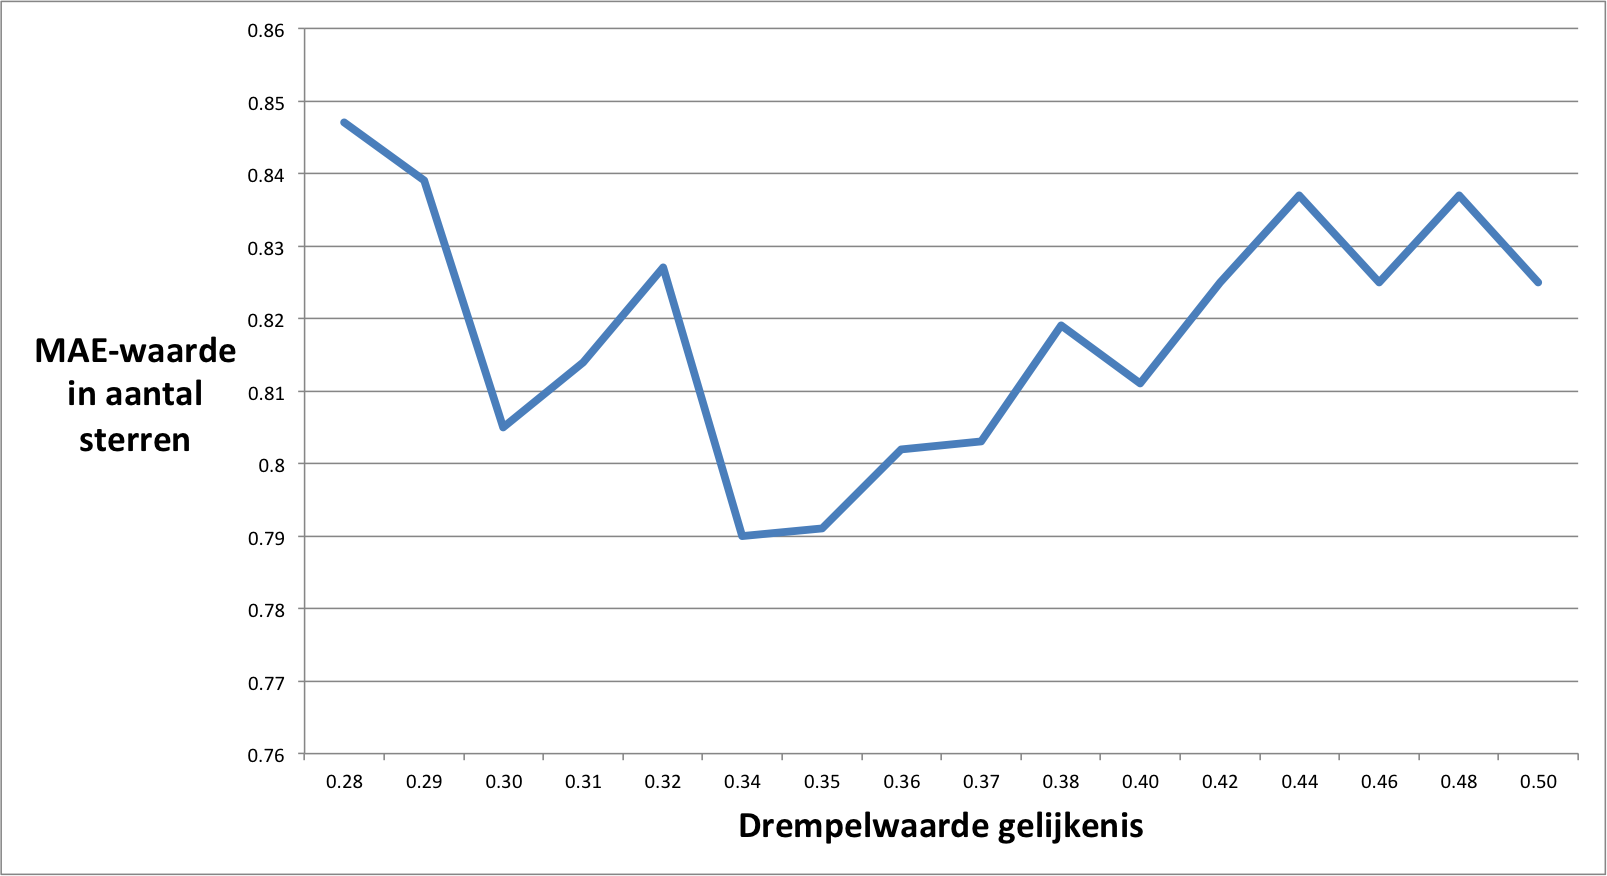
\includegraphics[width=\textwidth]{fig/mae}    
  \end{center}   
\end{figure}
   
\begin{figure}[htpb]   
    \label{Figuur::mse_rmse}      
  \begin{center}    
 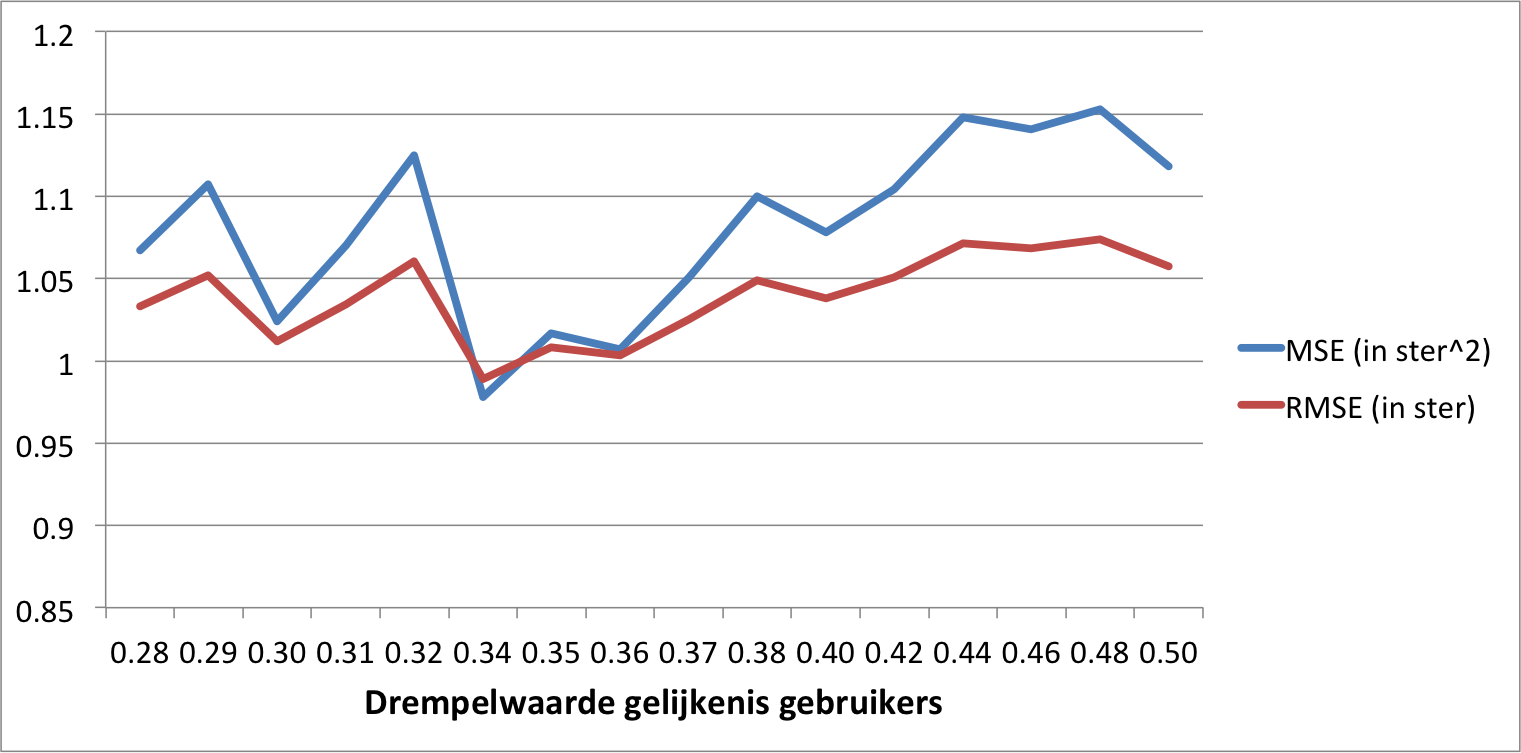
\includegraphics[width=\textwidth]{fig/mse_rmse}    
  \end{center}   
\end{figure}
   
\begin{figure}[htpb]   
    \label{Figuur::failed}      
  \begin{center}    
 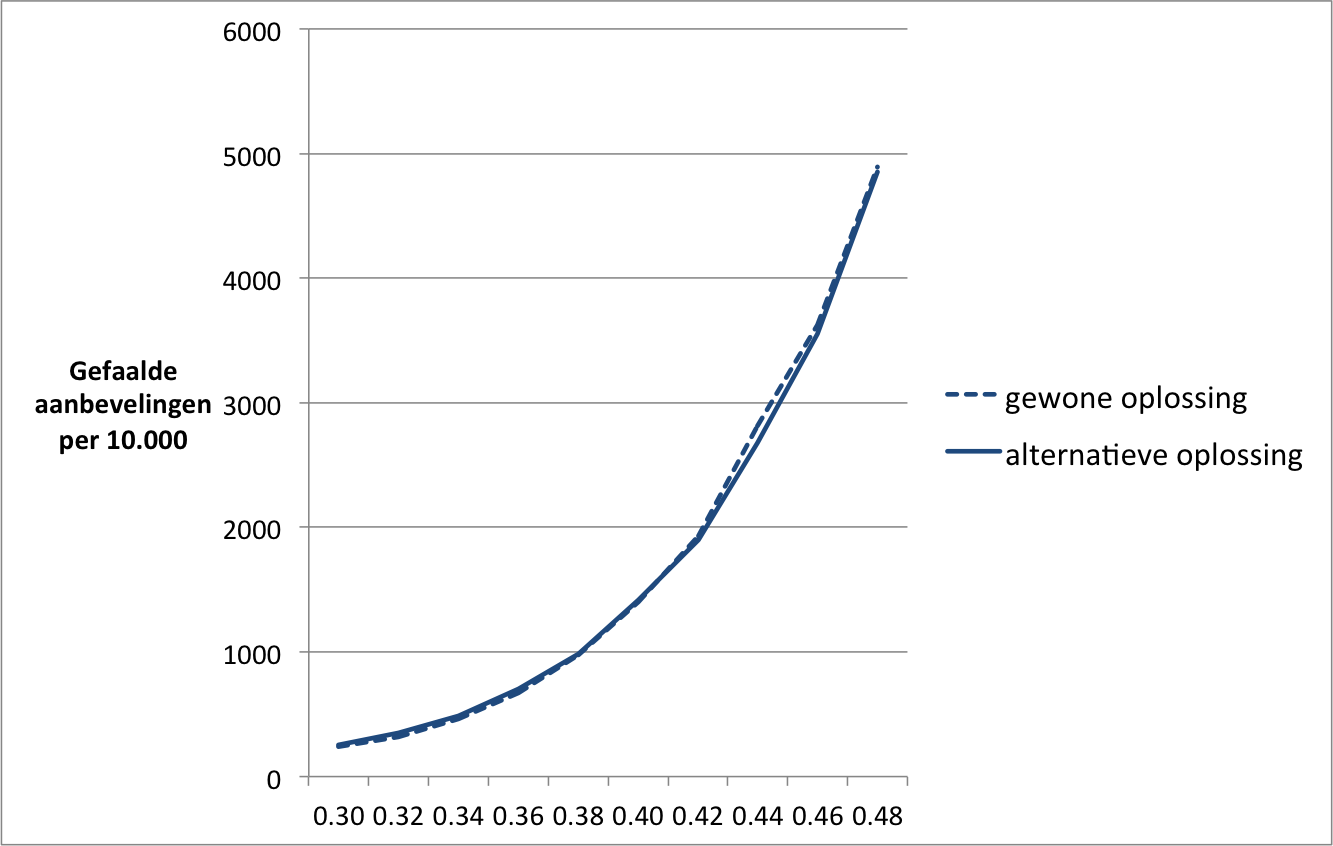
\includegraphics[width=\textwidth]{fig/failed}    
  \end{center}   
\end{figure}

\begin{figure}[htpb]   
    \label{Figuur::usedratings}      
  \begin{center}    
 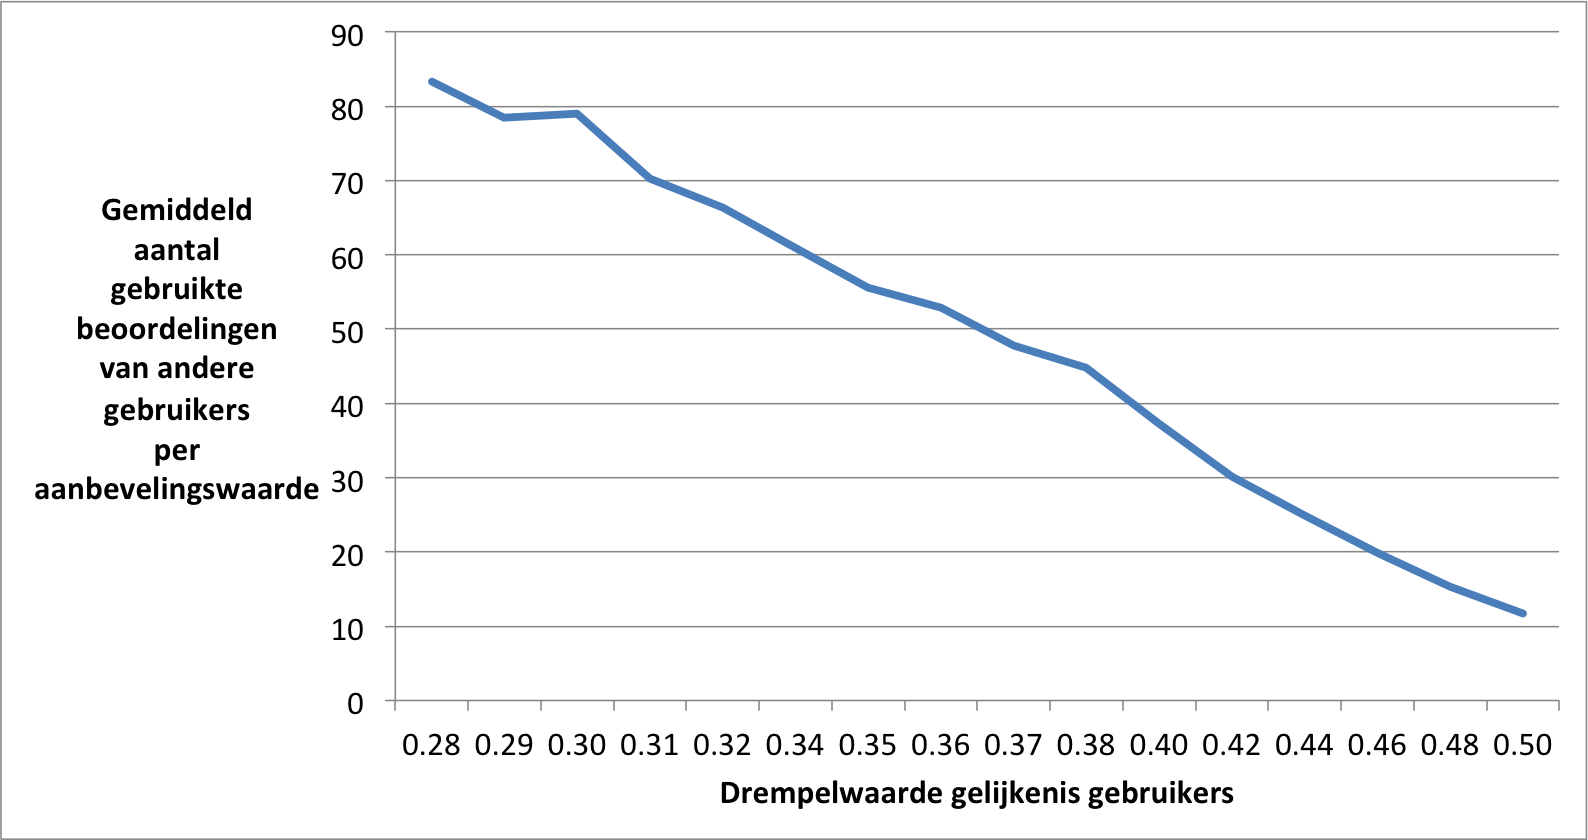
\includegraphics[width=\textwidth]{fig/usedratings}    
  \end{center}   
\end{figure}
Voor drempelwaarden groter dan 0.5 worden de aanbevelingen berekend op gemiddeld minder dan 10 beoordelingen van andere gebruikers, deze waarden zijn dus niet echt nuttig. Deze waarden leveren logischerwijs ook enorm veel gefaalde aanbevelingen. In de buurt van een drempelwaarde 0,34 \`a 0,35 worden de kleinste MAE, MSE en RMSEwaarden opgemeten. Met dit gegeven berekenden we de MAE, MSE en RMSE nogmaals voor een drempelwaarde van 0,345, ditmaal voor 10.000 beoordelingen. We bekwamen een MAE van 0,8057, een MSE van 1,0332 en een RMSE van 1,016. Deze MAE-waarde ligt vlakbij de MAE-waarde 0.7964 van de privacyvriendelijke oplossing uit "Svd-based collaborative filtering with privacy\cite{Polat:2005:SCF:1066677.1066860}" besproken in \ref{randomisatie}. De MAE voor een niet-privacyvriendelijke oplossing op deze dataset is 0,7146. Beide waarden werd berekend op identiek dezelfde dataset. De verschil van de bekomen MAE 0,8057 met de MAE van de niet-privacyvriendelijke methode 0,7146 is dus 0.0911 ster. Er wordt dus niet veel aan nauwkeurigheid ingeboet.
\subsection{Performantie}
\subsubsection{Het mobiele device}

\subsubsection{De aanbevelingsserver en de controleserver}